\documentclass{article}

\usepackage[spanish]{babel}
\usepackage[numbers,sort&compress]{natbib}
\usepackage{graphicx}
\usepackage{subfigure}
\usepackage{url}
\usepackage{amsmath}
\usepackage{hyperref}
\usepackage[top=15mm, bottom=40mm, left=15mm, right=15mm]{geometry}
\setlength{\parskip}{2mm}
\setlength{\parindent}{0pt}



\author{Dulce Esperanza Carrasco Castillo 1445183}
\title{Movimiento Browniano}
\date{\today}

\begin{document}

\maketitle


\section{Introducción}

Se le llama Moviniento Browniano al movimiento aleatorio que realiza una partícula en cierto entorno, en esta práctica se describe este movimiento mediante probabilidad. 

\section{Objetivo}
Introducir al uso de R por medio del Movimiento Browniano de una partícula y su probabilidad de regresar al origen.

\section{Descripción}
En un script en R (p1.R) se introduce el código proporcionado por la práctica, se ajusta el código a las específicaciones que se piden en este caso se requieren de 1 a 8 dimensiones, con caminatas de potencias de 2 con exponentes de 6 a 12 y con 30 repeticiones para cada combinación, los resultados se interpretan en una gráfica donde la distancia es tipo Manhattan. \url{elisaweb}

\section{Resultados}

Se puede observar como va aumentando el límite de pasos (distancia máxima) y la variación de probabilidad entre dimensiones, las cuales muestran un comportamiento aleatorio. (\ref{figura 1})

\begin{figure}[htbp]
\centering
\subfigure[]{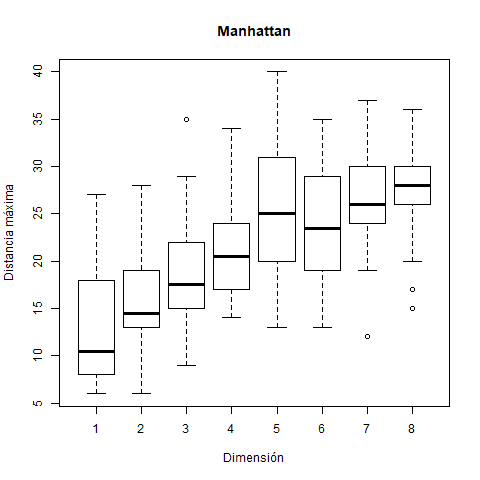
\includegraphics[width=46mm]{./man.png}}
\subfigure[]{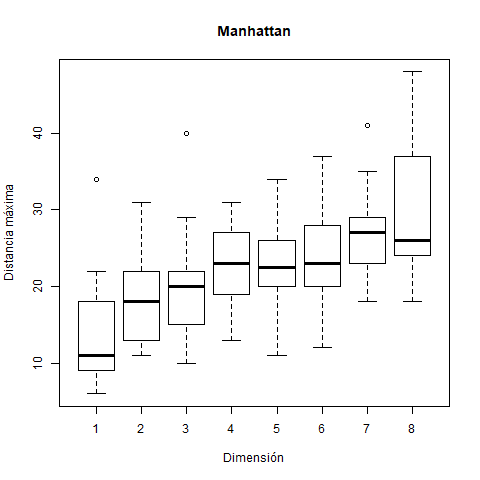
\includegraphics[width=46mm]{./27.png}}
\subfigure[]{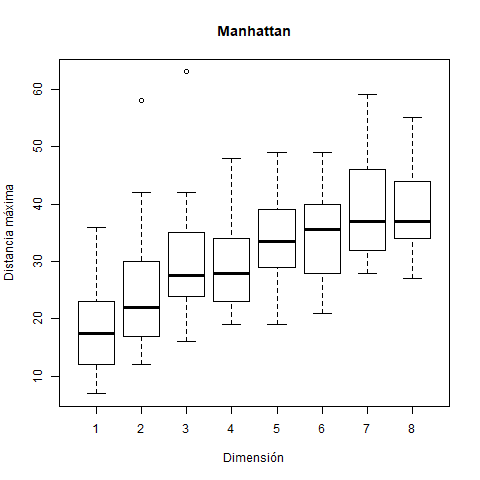
\includegraphics[width=46mm]{./28.png}}
\subfigure[]{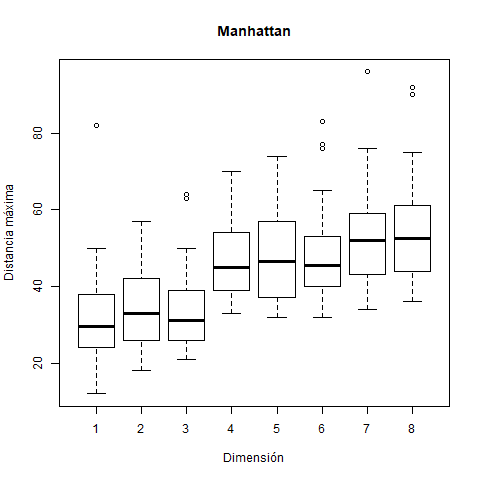
\includegraphics[width=46mm]{./29.png}}
\subfigure[]{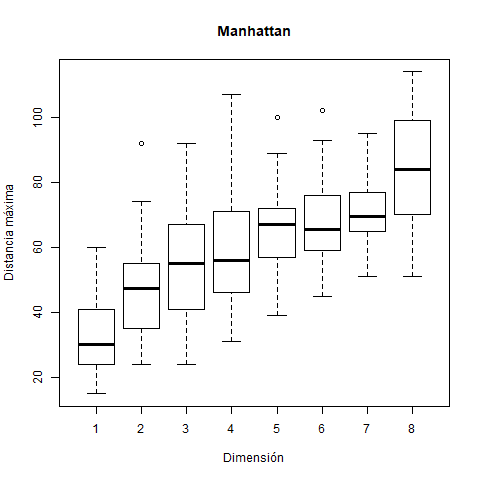
\includegraphics[width=46mm]{./210.png}}
\subfigure[]{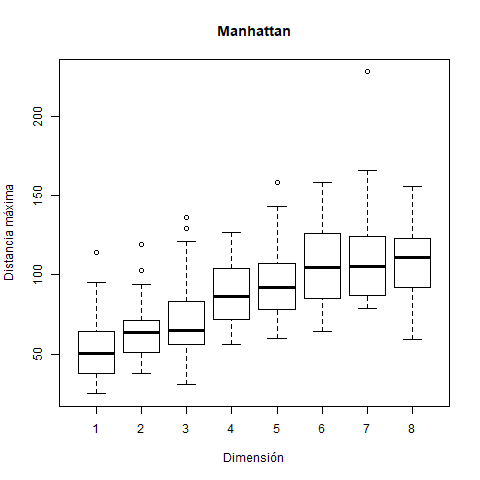
\includegraphics[width=46mm]{./211.png}}
\subfigure[]{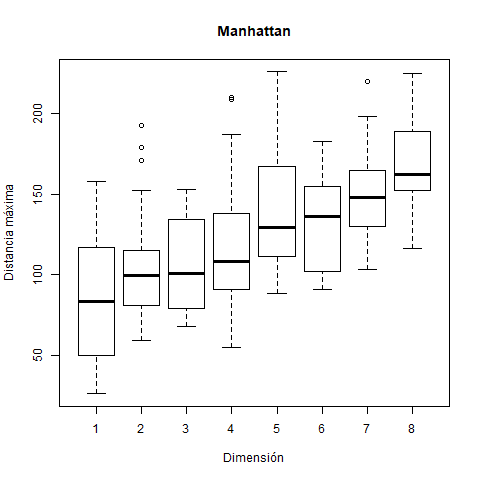
\includegraphics[width=46mm]{./212.png}}
\caption{Gráficas Manhattan} \label{figura 1}
\end{figure}









\bibliographystyle{plainnat}
\bibliography{biblio}

\end{document}
